\subsection{PieceWise Linear Discontinuous finite elements}
Next, we introduce the PieceWise Linear Discontinuous finite
elements developed in \cite{pwld_3d,pwld_2d}. The interest of PWLD finite
elements is that they can be used on arbitrary polygons. We will see in
Chapter \ref{mip_chapter} the advantages of using arbitrary polygons instead
of triangles or quadrilaterals. To obtain the PWLD basis
functions on two-dimensional polygons, we need to introduce the within-cell
point $c$. The coordinates of $c$ are weighted averages of the vertex coordinates:
\begin{align}
& x_c = \sum_{j=1}^{N_V} \alpha_{j} x_j\\
& y_c = \sum_{j=1}^{N_V} \alpha_{j} y_j
\end{align}
where $\sum_{j=1}^{N_V} \alpha_{j}=1$, $\alpha_j \geq 0\ \forall j$, and $N_V$ is 
the number of vertices of the cell.\\
The basis function at vertex $j$ is defined by \cite{pwld_2d}:
\begin{equation}
\chi_{j} (x,y) = t_{j}(x,y) + \alpha_j t_c(x,y)
\end{equation}
where the $t_j$ function is the linear functions such that $t_j (x,y)$ is
unity at vertex $j$ and zero at the  $j-1$, $j+1$, and $c$. The function 
$t_c(x,y)$ is unity at $c$ and zero at each vertex. In this work, the arbitrary 
positive weights $\alpha_j$ are chosen to be $\frac{1}{N_V}$. On a square cell with 
$\alpha_{j}=\frac{1}{4}\ \forall j$, the basis functions are given in Figure 
(\ref{pwld}):
\begin{figure}[H]
\centering
\subfloat[First basis function]{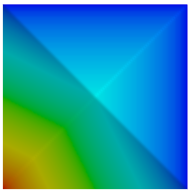
\includegraphics[width=0.25\textwidth]
  {./Spatial_discretizations/pwld_1}}
\subfloat[Second basis function]{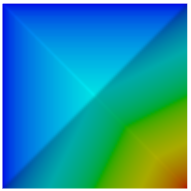
\includegraphics[width=0.25\textwidth]
  {./Spatial_discretizations/pwld_2}}\\
\subfloat[Third basis function]{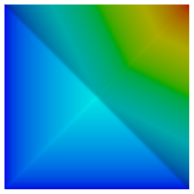
\includegraphics[width=0.25\textwidth]
  {./Spatial_discretizations/pwld_3}}
\subfloat[Fourth basis function]{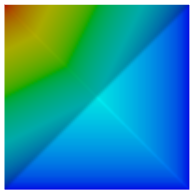
\includegraphics[width=0.25\textwidth]
  {./Spatial_discretizations/pwld_4}}
\caption{PWLD basis function}
\label{pwld}
\end{figure}
On triangular cells, the PWLD basis functions reduces to the standard Linear
Discontinuous (LD) basis functions if $\alpha_j = \frac{1}{3}$. 

Given the definition of the PWLD finite elements, it may seem complicated to
build the mass matrix, $\bs{M}$, or the gradient matrix, $\bs{G}$, on an 
arbitrary polygonal cells. The construction of such matrices can be greatly 
simplified using ``side'' sub-cells. A ``side'' sub-cell is a triangular cell 
made from two adjacent vertices and the point $c$. On each ``side'' sub-cells, 
the mass matrix, for example, can be build using LD finite elements. To do so, 
we first need to rewrite the mass matrix $\bs{M}$:
\begin{equation}
  \bs{M} = \sum_{k=1}^{N_V} \int_{S_k} \chi_i \chi_j\ d\br
\end{equation}
where $S_k$ are the ``side'' sub-cells (see Figure \ref{fig_sub_cell}). We see 
that $\bs{M}$ can be built by looping over all the ``side'' sub-cells. For a 
given ``side'' sub-cell $S_k$, we have:
\begin{equation}
  \int_{S_k} \chi_i \chi_j\ d\br = \int_{S_k} \(t_i t_j + \alpha
  t_i t_c + \alpha t_c t_i + \alpha^2 t_c^2\) d\br
\end{equation}
On $S_k$, the basis function $t_i$, $t_j$, and $t_c$, are identical to the LD
basis function. Therefore, if we note $\bs{M}_{S_k}$, the mass matrix on the 
``side'' sub-cell formed by the vertices 0, 1, and $c$:
\begin{figure}[H]
  \centering
  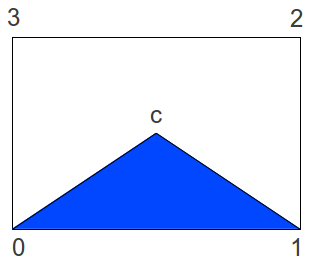
\includegraphics[width=0.3\textwidth]{./Spatial_discretizations/mass_matrix}
  \caption{Sub-cell (in blue) in the cell}
  \label{fig_sub_cell}
\end{figure}
$\bs{M}$ can be built using $\bs{M}_{S_k}$:
{\allowdisplaybreaks
\begin{align}
  & \bs{M}(0,0) =  \bs{M}_{S_k}(0,0) + \alpha \bs{M}_{S_k}(0,2) + \alpha
  \bs{M}_{S_k}(2,0) + \alpha^2 \bs{M}_{S_k}(2,2)\\
  & \bs{M}(0,1) =  \bs{M}_{S_k}(0,1) + \alpha \bs{M}_{S_k}(0,2) + \alpha
  \bs{M}_{S_k}(2,1) + \alpha^2 \bs{M}_{S_k}(2,2)\\
  & \bs{M}(0,2) =  \alpha \bs{M}_{S_k}(0,2) + \alpha^2 \bs{M}_{S_k}(2,2)\\
  & \bs{M}(0,3) =  \alpha \bs{M}_{S_k}(0,2) + \alpha^2 \bs{M}_{S_k}(2,2)\\
  & \bs{M}(1,0) =  \bs{M}_{S_k}(1,0) + \alpha \bs{M}_{S_k}(1,2) + \alpha
  \bs{M}_{S_k}(2,0) + \alpha^2 \bs{M}_{S_k}(2,2)\\
  & \bs{M}(1,1) =  \bs{M}_{S_k}(1,1) + \alpha \bs{M}_{S_k}(1,2) + \alpha
  \bs{M}_{S_k}(2,1) + \alpha^2 \bs{M}_{S_k}(2,2)\\
  & \bs{M}(1,2) =  \alpha \bs{M}_{S_k}(1,2) + \alpha^2 \bs{M}_{S_k}(2,2)\\
  & \bs{M}(1,3) =  \alpha \bs{M}_{S_k}(1,2) + \alpha^2 \bs{M}_{S_k}(2,2)\\
  & \bs{M}(2,0) =  \alpha \bs{M}_{S_k}(2,0) + \alpha^2 \bs{M}_{S_k}(2,2)\\
  & \bs{M}(2,1) =  \alpha \bs{M}_{S_k}(2,1) + \alpha^2 \bs{M}_{S_k}(2,2)\\
  & \bs{M}(2,2) =  \alpha^2 \bs{M}_{S_k}(2,2)\\
  & \bs{M}(2,3) =  \alpha^2 \bs{M}_{S_k}(2,2)\\
  & \bs{M}(3,0) =  \alpha \bs{M}_{S_k}(2,0) + \alpha^2 \bs{M}_{S_k}(2,2)\\
  & \bs{M}(3,1) =  \alpha \bs{M}_{S_k}(2,1) + \alpha^2 \bs{M}_{S_k}(2,2)\\
  & \bs{M}(3,2) =  \alpha^2 \bs{M}_{S_k}(2,2)\\
  & \bs{M}(3,3) =  \alpha^2 \bs{M}_{S_k}(2,2). 
\end{align}}    
To finish to build $\bs{M}$, we need to loop over all of the ``side''
sub-cells, $S_k$ ($k=1,\hdots,N_v$), of the cell. The gradient matrix is built 
similarly.

\section{Conclusions}
In this section, we explained how Source Iteration, Krylov solvers, and
Diffusion can be used to solve the transport equation. The two spatial
discretization, BLD and PWLD finite elements, that we will employ in the next
Chapters have been presented.
